\documentclass[12pt, titlepage]{article}

\usepackage{booktabs}
\usepackage{tabularx}
\usepackage{hyperref}
\usepackage{amssymb, amsmath}
\usepackage{enumerate}
\usepackage{mdframed}
\usepackage{color}
\usepackage{soul}
\usepackage{framed}
\usepackage{siunitx}
\usepackage{graphicx}


\usepackage[round]{natbib}

\title{Carbon Charts: Software Requirements Specification\\}


\author{
    McMaster University\\
    Group 18 \\
    Darsi Anandarajah \\
    Justin Licari \\
    Eliad Moosavi \\
    Thomas Mullen \\
    Richard Zhang \\
}


\date{\today}

\begin{document}

\maketitle

\pagenumbering{roman}
\tableofcontents
\listoftables
\listoffigures

\begin{table}[bp]
\caption{\bf Revision History}
\begin{tabularx}{\textwidth}{p{3cm}p{2cm}X}
\toprule {\bf Date} & {\bf Version} & {\bf Notes}\\
\midrule
October 30, 2018 & 1.0 & Created document, REV-0\\

\bottomrule
\end{tabularx}
\end{table}

\newpage

\pagenumbering{arabic}

%----------------------------------------------------------------------------------------
%	Introduction
%----------------------------------------------------------------------------------------
\section{Introduction}
This document outlines the software requirements for Carbon Charts. The purpose of this document is to specify requirements and provide a complete description of the library to be developed. It will outline the intended purpose, features of the library, behavior, and general factors that affect its requirements. Additionally, it will illustrate the constraints under which the library must operate and conform to. This document will serve as a complete declaration of the data visualization library in development and is intended for stakeholders and the library developers, Group 18. The audience includes the stakeholders, Dr. Wassyng, Nicholas Annable, Joshua Barkovic, Spencer Deevy, Viktor Smirnov and any potential developers. 


%//FIGURE OUT HOW TO DEFINE HARDWARE ASAP  
%In addition, it outlines the hardware requirements relating to acquiring the real-time sensory data that will be displayed by the charts.

%----------------------------------------------------------------------------------------
%	PROJECT DRIVERS
%----------------------------------------------------------------------------------------
\section{Project Drivers}
\subsection{Background of the Project Effort}
The information age had led to a rapid increase in the amount of raw data available. This increase in raw data is only beneficial when we use methods to derive insights from it. Humans are visual creatures, detecting patterns in sets of data is more easily interpreted using data visualization techniques. A common and convenient mode of consuming visualized data is through graphical charts. The process of mapping information to visuals is more efficient and accurate when employing the power of computing. The increased speed enables the use of much larger data sets while allowing for quick re-rending of alternative mappings. The added benefits through computing drove application developers and organizations such as IBM Canada to highlight the need for a consistent data visualization framework.  

%//FIX THIS 
%The capabilities of the library will be visualized by charting real-time sensory data, such as temperature, pressure, proximity etc.

\subsection{Scope}
Carbon Charts is an open-source JavaScript data visualization library that will be used as a functional component of IBM's Carbon Design System. The library is expected to comply with the general IBM design guidelines with the intended goal of making any data visualization processes within their products more efficient while eliminating duplicated work within different teams. It will be used to extend the data visualization capabilities of IBM Carbon Design System by serving as an interactive, lightweight charting library. Additionally, it should be designed in accordance with design principles that follow its open source nature. 

\subsubsection{Benefits}
The proposed library merits the following benefits:
\begin{itemize}
    \item Reuseability: The Carbon Charts library will allow for the use of its existing (stable and verified) visualization techniques within the software development process of other internal IBM products,  
    \item Extensibility: As an open-source project, the library is easily extensible and provides for change while minimizing the impact to existing system functions. High cohesion and loose coupling allow for continual development with-in the open-source community.
    
    %--> Design principle that we can use for the design doc, so leave reference here.
    %\item Liskov's Substitution Principle: Every chart in the Carbon Charts Library inherently derived from a base chart class.  \item Separation of Concerns: Carbon Charts separates the logic of content presentation style and that of how the content interacts and behaves with the user. 
    
\end{itemize}

\subsection{The Stakeholders}
\subsubsection{IBM Canada Ltd}
\begin{itemize}

%//Note: we should define distruptive innovation just incase 
    \item IBM Canada is generally interested in disruptions within the open-source community, they invest significant amounts of effort and funds into creating an inspirational footprint within the community.
   
 %//Note:  (reference stole it from carbon design system facts)
    \item Carbon the new IBM Design Language will define and guide everything designed by IBM, including software products, digital and traditional marketing, hardware, advertising. and more. 
    
    
    %\item The library is expected to comply with the general IBM design guidelines with the intended goal of making any data visualization processes within their products more efficient while eliminating duplicated work within different teams.
\end{itemize}

\subsubsection{Application Developers}
\begin{itemize}
    \item Web application developers can use the library to create interactive visualizations of data they would like to present to their users.  
    \item Generally, developers would be looking for a solution that is lightweight, high-performance, reliable and accurate in results. Depending on what organization or project they are involved in, they might also have accessibility and internationalization requirements.
\end{itemize}


\subsubsection{Application Users}
\begin{itemize}
    \item Users of web applications represent the target audience of this library. They can use charts generated by the developer and through the library, to monitor data (sensitive data in many cases), analyze patterns between data sets, make decisions based on historic representations and values, all while being able to take advantage of real-time visualizations in some cases (e.g. trading).
    \item Users will generally be looking for reliable functionality, an appealing visual representation and accessibility.
\end{itemize}
\subsection{Naming Conventions and Terminology}
\begin{itemize}
    \item \textbf{Axis Chart:} Axis charts display data between a set of axis. Axis charts are 2 or 3 dimensional, with at least an x and y axis.
    \item \textbf{Non-Axis Chart:} Axis charts display data within an area not defined by axis. (e.g. Pie Charts).
    \item \textbf{Right-to-Left Support:} The ability to display languages that read right to left, such as Farsi.
    \item \textbf{Browser Tiers:} We define two tiers of browsers A and B. Tier A browsers consist of the two latest versions of Chrome, Firefox, Opera and Safari at any time, and any versions below those including IE-11+ will be part of tier B.
    \item \textbf{Test Data:} A set of example data. This set will initially consist of a random sampling of all valid data within the expected range, but will be extended to any particular data that cause issues in the software as it develops. Requirements that involve the test data in their fit criterion will be considered unmet if any member of the test data fail that requirement.
    \item \textbf{Demonstration Environment:} An environment resembling a common household room; no extreme conditions (temperature, pressure, magnetic fields, impact forces etc).
\end{itemize}
\subsection{References}
\begin{enumerate}
    \item Murray, Scott. Interactive Data Visualization for the Web. O'Reilly, 2013.
    \item D. L. Parnas, P. C. Clements, A rational design process: How and why to fake it, IEEE Transactions on Software Engineering, v.12 n.2, p.251-257, Feb. 1986
\end{enumerate}
\subsection{Constraints}
\subsubsection{Solution Constraints}
\begin{itemize}
    \item Must adhere to IBM open source guideline (eg. code styling, structure).
    \item Must operate as a component within IBM's Carbon Design System.
\end{itemize}

\subsubsection{Schedule Constraints}
\begin{itemize}
    \item Milestone deadlines for McMaster Capstone project.
    \item Release deadlines for external IBM projects that rely on stable versions of Carbon Charts. These deadlines may be announced at any time in the future.
    \item Due to team members having other obligations, the project is limited to 10 hours per week. Team members may opt to exceed this limit, but it is not required.
\end{itemize}

\subsubsection{Budget Constraints}
\begin{itemize}
    \item \$750 CAD is the budget constraint imposed on us by the assigment.
\end{itemize}

\section{Off-The-Shelf Solutions}
\begin{itemize}
    \item d3.js is a widely used JavaScript library for data visualization. Initially released in 2011, it has gone through many levels of user testing, bug discoveries and refactors, and has iterated to become an industry standard for web visualizations. The library offers some core functionality to be able to select and manipulate SVG elements, implement quick and easy progressive web transitions, perform data-binding on DOM elements etc.
    \item Chart.js is an open source JavaScript charting library for designers and developers.
    \item Chartist.js an open source JavaScript charting library. It is the product of a community that was disappointed about the abilities provided by other charting libraries.
    \item (Hardware) Arduino is an open-source electronic prototyping platform enabling users to create interactive electronic objects. It can be used to interface with various sensors.
\end{itemize}

\subsection{Relevant Facts and Assumptions}
\subsubsection{Facts}
\begin{itemize}
    \item Data representations are often only defined for specific data types. For example, it is obvious that charts with numeric axis can only accept numerical values on that axis. It will always be assumed that any such invalid data is not present.
    \item Data sets are unbounded in size and can have any number of elements. We will assume an "expected data range" of 0 to 50 data points. Data sets larger than this cannot be usefully displayed in a visual graph due to screen space limitations. This is a strict limit which allows for application developers using this library to define how large sets of data are mapped.    
    \item The hardware will only be expected to operate in the demonstration environment.
\end{itemize}

\subsubsection{Assumptions}
\begin{itemize}
    \item It is assumed that developers will use library functions correctly, and pass in the correct data types within the correct data range.
\end{itemize}

%---------------------------------------------------------------------------------------
%	Context Diagrams
%----------------------------------------------------------------------------------------
\subsection{Context Diagrams}
The following context diagram defines the boundaries of the system and the entities that act with it. 
%\begin{figure}[h!]
%\centering
%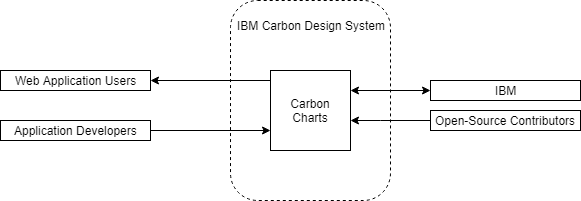
\includegraphics[scale=0.7]{context.png}
%\caption{Context Diagram showing the bounds of the library in development. }
%\label{fig:context}
%\end{figure}

%\section{Rev-1 Functional Requirements}
%\subsection{Functional Requirements}


 %   \begin{tabular}{ | l | l | p{12cm} |}
 %   \hline
 %   Identifier & Priority & Requirement \\ \hline
 %   REQ1 & 1 & The developer must be able to render a list of data or values as a chart   \\ \hline
    
%\end{tabular}


%---------------------------------------------------------------------------------------
%	FUNCTIONAL REQUIREMENTS 
%----------------------------------------------------------------------------------------
\section{Functional}
%type of graphs we are ensuring functionality and IBM design principles for 
%Bar chart -> stack chart and grouped chart
%Ciricle Chart -> pie and donue chart 
% 
%----------------------------------------------------------------------------------------
%	IBM, Library and Open-Source Requirements
%----------------------------------------------------------------------------------------
\subsection{IBM and Library Requirements}
\begin{flushleft}
\textbf{Requirement \#: FN-1} \\
\textbf{Description:} The developer can render a list of data and a list of values as a chart.  \\
\textbf{Rational:} Basic functionality. \\
\textbf{Fit Criterion:} For any chart type, the test data can be rendered. \\
\textbf{Stakeholders:} Application Developers, IBM Canada Ltd \\ 
\end{flushleft}
\begin{flushleft}
\textbf{Requirement \#: FN-2} \\
\textbf{Description:} The developer can choose the type of chart to be displayed. \\
\textbf{Rational:} Basic functionality. \\
\textbf{Fit Criterion:} For all charts types, the test data can be rendered. \\
\textbf{Stakeholders:} Application Developers, IBM Canada Ltd\\
\end{flushleft}
\begin{flushleft}
\textbf{Requirement \#: FN-3} \\
\textbf{Description:} Subsection colours must match the colour corresponding to that subsection legend entry. \\
\textbf{Rational:} Legend entries must be visually connected to their data without requiring text. \\
\textbf{Fit Criterion:} Visual confirmation of rendered test data and legend. \\
\textbf{Stakeholders:} Application Users, Application Developers, IBM Canada Ltd\\
\end{flushleft}
\begin{flushleft}
\textbf{Requirement \#: FN-4} \\
\textbf{Description:} All data points in axis charts must be directly vertical of the x-axis tick correlating to that point's label and directly horizontal of the y-axis tick corresponding to that point's value. \\
\textbf{Rational:} This allows data to be immediately correlated with it's corresponding axis values. \\
\textbf{Fit Criterion:} Visual confirmation of rendered test data. \\
\textbf{Stakeholders:} Application Users, Application Developers, IBM Canada Ltd\\
\end{flushleft}
\begin{flushleft}
\textbf{Requirement \#: FN-5} \\
\textbf{Description:} The user has the option to save a graph as an SVG image. \\
\textbf{Rational:} Allows the user to export the graph without requiring them to use a screenshot tool. \\
\textbf{Fit Criterion:} SVG image is visually similar to rendered graph. \\
\textbf{Stakeholders:} Application Users \\
\end{flushleft}
\begin{flushleft}
\textbf{Requirement \#: FN-6} \\
\textbf{Description:} Library must respect The right-to-left preference in a user's browser and display text right-to-left. \\
\textbf{Rational:} Not all users read left-to-right. \\
\textbf{Fit Criterion:} All other requirements are met when rendering text right-to-left. \\
\textbf{Stakeholders:} Application Users \\
\end{flushleft}
\begin{flushleft}
\textbf{Requirement \#: FN-7} \\
\textbf{Description:} The developer shall bell able to specify a rectangular region behind an axis chart can be displayed. \\
\textbf{Rational:} This is a common way to indicate a special region of the data to the user. \\
\textbf{Fit Criterion:} Visual confirmation of rendered test data with a threshold. \\
\textbf{Stakeholders:} Application Users, Application Developers, IBM Canada Ltd \\
\end{flushleft}
\begin{flushleft}
\textbf{Requirement \#: FN-8} \\
\textbf{Description:} The user can adjust the graph viewpoints, making data larger or smaller and changing the visible region. Axis and legends should remain where they are. \\
\textbf{Rational:} Many data sets have a variety of scale and need to be explored from multiple viewpoints. \\
\textbf{Fit Criterion:} The user can zoom and scroll the rendered test data. \\
\textbf{Stakeholders:} Application Users, Application Developers, IBM Canada Ltd \\
\end{flushleft}
\begin{flushleft}
\textbf{Requirement \#: FN-9} \\
\textbf{Description:} The developer can disable any visual elements of the software for their application. \\
\textbf{Rational:} Some elements may be unnecessary or unwanted, depending on the application. \\
\textbf{Fit Criterion:} Given any visual element, it can be removed by the developer. \\
\textbf{Stakeholders:} Application Developers \\
\end{flushleft}
\begin{flushleft}
\textbf{Requirement \#: FN-10} \\
\textbf{Description:} The users ability to resize any chart should be limited to the minimum and maximum scale size of a chart.  \\
\textbf{Rational:} Developers may want to enforce a viewing scale that they believe is appropriate for the data. \\
\textbf{Fit Criterion:} If a minimum or maximum scale size limit is enabled on a chart rendering the test data, a user cannot scale past that limit. \\
\textbf{Stakeholders:} Application Developers \\
\end{flushleft}
\begin{flushleft}
\textbf{Requirement \#: FN-11} \\
\textbf{Description:} Transitions made by selecting legend items should correctly adjust the chart, load data and generate elements using the selected data sets. \\
\textbf{Rational:} Users should not lose any data due to chart transitions. This is a common problem in charting applications. \\
\textbf{Fit Criterion:} All test data is still visible after a transition, unless it was explicitly hidden. \\
\textbf{Stakeholders:} Application Users, Application Developers \\
\end{flushleft}

%----------------------------------------------------------------------------------------
%	Bar Chart Requirements (regular, stacked and grouped)
%----------------------------------------------------------------------------------------
\subsection{Bar Chart : Stack and Grouped}
\begin{flushleft}
\textbf{Requirement \#: FN-12} \\
\textbf{Description:} Data can be rendered as rectangular subsections which originate from an x axis, and stretch upward.  \\
\textbf{Rational:} Definition of a correct bar chart. \\
\textbf{Fit Criterion:} Visual confirmation of rendered test data. \\
\textbf{Stakeholders:} Application Users, Application Developers, IBM Canada Ltd\\
\end{flushleft}
\begin{flushleft}
\textbf{Requirement \#: FN-13} \\
\textbf{Description:} Data can be rendered as multiple series of stacked rectangular subsections which originate from an x axis, and stretch upward.  \\
\textbf{Rational:} Definition of a correct stacked bar chart. \\
\textbf{Fit Criterion:} Visual confirmation of rendered test data. \\
\textbf{Stakeholders:} Application Users, Application Developers, IBM Canada Ltd\\
\end{flushleft}

%----------------------------------------------------------------------------------------
%	Chart Type: Circle Charts Pie, Donut and Bubble)
%----------------------------------------------------------------------------------------
\subsection{Circle Charts : Pie, Donut and Bubble}
\begin{flushleft}
\textbf{Requirement \#: FN-14} \\
\textbf{Description:} Data can be rendered as a circle is divided into subsections which stretch from the outer radius to the center.(this is a separate requirement) Each subsection is assigned a different colour. \\
\textbf{Rational:} Definition of a correct pie chart. \\
\textbf{Fit Criterion:} Visual confirmation of rendered test data. \\
\textbf{Stakeholders:} Application Users, Application Developers, IBM Canada Ltd\\
\end{flushleft}

\begin{flushleft}
\textbf{Requirement \#: FN-15} \\
\textbf{Description:} Data can be rendered as a circle is divided into subsections which stretch from border to center. Each subsection is assigned a different colour.  \\
\textbf{Rational:} Definition of a correct donut chart. \\
\textbf{Fit Criterion:} Visual confirmation of rendered test data. \\
\textbf{Stakeholders:} Application Users, Application Developers, IBM Canada Ltd\\
\end{flushleft}
%----------------------------------------------------------------------------------------
%	Chart Type: Circle Charts Pie, Donut and Bubble)
%----------------------------------------------------------------------------------------
\subsubsection{Pie and Donut Charts}
\begin{flushleft}
\textbf{Requirement \#: FN-16} \\
\textbf{Description:} A perpendicular X and Y axis is displayed, unless the developer explicitly excludes this feature or the chart is a pie or donut chart. \\
\textbf{Rational:} Definition of a correct axis chart. \\
\textbf{Fit Criterion:} Visual confirmation of rendered test data and axis. \\
\textbf{Stakeholders:} Application Users, Application Developers, IBM Canada Ltd\\
\end{flushleft}
\begin{flushleft}
\textbf{Requirement \#: FN-17} \\
\textbf{Description:} The maximum number of subsections in a pie or donut chart is 7. If the number of subsections exceeds this, the smallest subsections will be collapsed into an "other" subsection until there are only 7 subsections. \\
\textbf{Rational:} It is desirable to simplify these chart types. \\
\textbf{Fit Criterion:} Visual confirmation of rendered test data with <7, 7, and >7 subsections. \\
\textbf{Stakeholders:} Application Users, Application Developers, IBM Canada Ltd\\
\end{flushleft}
\begin{flushleft}
\textbf{Requirement \#: FN-18} \\
\textbf{Description:} Each data point in a pie or donut chart is displayed with an area proportional to that data point's absolute value divided by the sum of all data points. \\
\textbf{Rational:} Absolute data should be renormalized in these chart types to fit the available display area. \\
\textbf{Fit Criterion:} Visual confirmation of rendered test data. \\
\textbf{Stakeholders:} Application Users, Application Developers, IBM Canada Ltd\\
\end{flushleft}
\subsubsection{Bubble Charts}
\begin{flushleft}
\textbf{Requirement \#: FN-19} \\
\textbf{Description:} Bubble Charts must consist of ovular or circular subsections within the boundaries of the x and y axis. Individual subsections must be one consistent colour.  \\
\textbf{Rational:} Definition of a correct bubble chart. \\
\textbf{Fit Criterion:} Visual confirmation of rendered test data. \\
\textbf{Stakeholders:} Application Users, Application Developers, IBM Canada Ltd\\
\end{flushleft}

%----------------------------------------------------------------------------------------
%	Line Chart Requirements
%----------------------------------------------------------------------------------------
\subsection{Line Chart}
\begin{flushleft}
\textbf{Requirement \#: FN-20} \\
\textbf{Description:} Data can be rendered as coordinates plotted on an x and y grid, connected by a line. \\
\textbf{Rational:} Definition of a correct line chart. \\
\textbf{Fit Criterion:} Visual confirmation of rendered test data. \\
\textbf{Stakeholders:} Application Users, Application Developers, IBM Canada Ltd\\
\end{flushleft}

%----------------------------------------------------------------------------------------
%	Area Chart Requirements 
%----------------------------------------------------------------------------------------
\subsection{Area Chart}
\begin{flushleft}
\textbf{Requirement \#: FN-21} \\
\textbf{Description:} Area chart subsections must be within the boundaries of the x and y axis. Individual subsections must be one consistent colour.  \\
\textbf{Rational:} Definition of a correct area chart. \\
\textbf{Fit Criterion:} Visual confirmation of rendered test data. \\
\textbf{Stakeholders:} Application Users, Application Developers, IBM Canada Ltd\\
\end{flushleft}

\subsection{Hardware Requirements}
\begin{flushleft}
\textbf{Requirement \#: FN-22} (Hardware) \\
\textbf{Description:} The hardware component records real-time sensory data, including temperature, pressure, and proximity.and is displayed using the charts.  \\
\textbf{Fit Criterion:} Data recorded by the sensors accurately reflects the demonstration environment. \\
\textbf{Stakeholders:} Application Users \\
\end{flushleft}
\begin{flushleft}
\textbf{Requirement \#: FN-23} (Hardware) \\
\textbf{Description:} The hardware component can transfer data to the display device and the data is displayed using the software's charts.  \\
\textbf{Fit Criterion:} Demonstration data from the hardware component is accurately displayed in a chart. \\
\textbf{Stakeholders:} Application Users \\
\end{flushleft}


%----------------------------------------------------------------------------------------
%	NON FUNCTIONAL REQUIREMENTS
%----------------------------------------------------------------------------------------
\section{Non-Functional}
\subsection{Look and Feel}
\begin{flushleft}
\textbf{Requirement \#: LF-1} \\
\textbf{Description:} All animations must rendered smoothly. \\
\textbf{Rational:} Jittery animations can interfere with data interpretation. \\
\textbf{Fit Criterion:} Visual affirmation of rendered and animated test data.
\textbf{Stakeholders:} Application Users \\
\end{flushleft}
\begin{flushleft}
\textbf{Requirement \#: LF-2} \\
\textbf{Description:} Color Maps or the palettes used should adhere to IBM design color specs separating palettes by standard qualitative and high contrast qualitative. \\
\textbf{Rational:}IBM Design guidelines and defined coloring principles. \\
\textbf{Fit Criterion:} Visual affirmation of rendered test data.  \\
\textbf{Stakeholders:} Application Developers and Users \\
\end{flushleft}
\begin{flushleft}
\textbf{Requirement \#: LF-3} \\
\textbf{Description:} X-axis must always be positioned at the bottom of the chart with the labels rotated -\ang{45} by default and aligned to the right of the y-axis. \\ 
\textbf{Rational:} IBM Design guidelines and defined coloring principles.\\
\textbf{Fit Criterion:} Visual affirmation of rendered test data. \\
\textbf{Stakeholders:} Application Developers and Users \\
\end{flushleft}
\begin{flushleft}
\textbf{Requirement \#: LF-4} \\
\textbf{Description:} Y-axis must display no more than 6-digit metrics on a single axis. Separate multiple metric title labels with commas. \\ 
\textbf{Rational:} IBM Design guidelines and defined coloring principles. \\
\textbf{Fit Criterion:} Visual affirmation of rendered test data. \\
\textbf{Stakeholders:} Application Developers and Users \\
\end{flushleft}

\subsection{Usability}
\begin{flushleft}
\textbf{Requirement \#: USB-1} \\
\textbf{Description:} Using a screen-reader, one should be able to navigate across all elements of a chart, and hear back information regarding labels and values corresponding to the element. \\
\textbf{Rational:} Carbon Charts should be usable by the widest possible range of users, including visually impaired individuals. \\
\textbf{Fit Criterion:} The rendered test data can be fully interpreted using JAWS screenreader. \\
\textbf{Stakeholders:} Application Users, IBM Canada Ltd \\
\end{flushleft}
\begin{flushleft}
\textbf{Requirement \#: USB-2} \\
\textbf{Description:} Charts and legends should be able to render using pattern fills rather than solid color fills in accessibility mode. \\
\textbf{Rational:} Visual accessibility is also important for visually impaired individuals, including individuals with colour blindness. Legend items should also follow the same logic. \\
\textbf{Fit Criterion:} The rendered test data can be fully interpreted in black-and-white. \\
\textbf{Stakeholders:} Application Users, IBM Canada Ltd \\
\end{flushleft}
\subsection{Safety}
Developers using this library should independently evaluate it's properties and how they relate to their system's safety requirements. Due to this software's intended use as a module within another application, it is not possible for us to provide safety guarantees without knowing the application's specific requirements. \\

We will make efforts to ensure documentation of the software is up-to-date and accurate to allow developers to make informed decisions on the suitability of this software for their application, in regards to safety or otherwise.

\subsection{Performance}
\begin{flushleft}
\textbf{Requirement \#: PERF-1} \\
\textbf{Description:} The compiled bundle size must be of a reasonable size. \\
\textbf{Rational:} The bundle should remain small to ensure quick load times. \\
\textbf{Fit Criterion:} The compiled bundle size must be less than 150kb, including compression.\\
\textbf{Stakeholders:} Application Users \\
\end{flushleft}
\begin{flushleft}
\textbf{Requirement \#: PERF-2} \\
\textbf{Description:} The render time of charts should be short. \\
\textbf{Rational:} The user will not want to wait long times for data to render. \\
\textbf{Fit Criterion:} The render time of a chart inside the expected data range should be 50ms without animations, and 800ms with animations. \\
\textbf{Stakeholders:} Application Users \\
\end{flushleft}
\begin{flushleft}
\textbf{Requirement \#: PERF-2} \\
\textbf{Description:} The software should not use a large amount of volatile memory. \\
\textbf{Rational:} Other applications running on the same page should not struggle with memory shortages due to the software. \\
\textbf{Fit Criterion:} The volatile memory footprint of the software does not exceed 3mB while rendering the test data.\\
\textbf{Stakeholders:} Application Users \\
\end{flushleft}
\begin{flushleft}
\textbf{Requirement \#: PERF-3} (Hardware) \\
\textbf{Description:} The hardware component records data values at a frequency of at least $100ms^{-1}$. \\
\textbf{Rational:} The data should be refreshed often enough that two chart refresh cycles do not pass without new data. \\
\textbf{Stakeholders:} Application Users \\
\end{flushleft}
\subsection{Installability}
\begin{flushleft}
\textbf{Requirement \#: INST-1} \\
\textbf{Description:} The software is installable with Node Package Manager. \\
\textbf{Rational:} Other applications running on the same page should not struggle with memory shortages due to the software. \\
\textbf{Fit Criterion:} The command npm install carbon-charts is sufficient to install the software.\\
\textbf{Stakeholders:} Application Developers \\
\end{flushleft}
\subsection{Operational}
\begin{flushleft}
\textbf{Requirement \#: OP-1} \\
\textbf{Description:} The software is supported by any operating system that supports Node.js. \\
\textbf{Rational:} Developers should not be limited by their operating system when deciding to use the software. \\
\textbf{Fit Criterion:} No operating system with at least \%2 market share is unsupported. \\
\textbf{Stakeholders:} Application Developers \\
\end{flushleft}
\begin{flushleft}
\textbf{Requirement \#: OP-2} \\
\textbf{Description:} The software is fully supported by all Tier A browsers. \\
\textbf{Rational:} Users with common browsers should not encounter issues.\\
\textbf{Fit Criterion:} None of the defined Tier A browsers are unsupported.\\
\textbf{Stakeholders:} Application Users, Application Developers, IBM Canada Ltd \\
\end{flushleft}
\begin{flushleft}
\textbf{Requirement \#: OP-3} \\
\textbf{Description:} The software is partially supported by all Tier B browsers. \\
\textbf{Rational:} An attempt should be made to support fallbacks for uncommon browsers in order to avoid excluding users. \\
\textbf{Fit Criterion:} All Tier B browsers can at least display the test data. \\
\textbf{Stakeholders:} Application Users, Application Developers, IBM Canada Ltd \\
\end{flushleft}

\subsection{Security}
\begin{flushleft}
\textbf{Requirement \#: SEC-1} \\
\textbf{Description:} The software must not utilize any deprecated or insecure dependencies. \\
\textbf{Rational:} The security of the software should not be compromised by a dependency. \\
\textbf{Fit Criterion:} No warnings should be present when the software is scanned using NPM's Node Security Platform. \\
\textbf{Stakeholders:} Application Users, Application Developers, IBM Canada Ltd \\
\end{flushleft}
\begin{flushleft}
\textbf{Requirement \#: SEC-2} \\
\textbf{Description:} The software must not make any external HTTP requests. \\
\textbf{Rational:} This reduces the cross-site scripting (XSS) attack surface. \\
\textbf{Fit Criterion:} No form of HTTP request code should be present in the software. \\
\textbf{Stakeholders:} Application Users, Application Developers, IBM Canada Ltd \\
\end{flushleft}
\subsection{Legal}
\begin{flushleft}
\textbf{Requirement \#: LGL-2} \\
\textbf{Description:} The software must meet IBM's arbitrary legal requirements. \\
\textbf{Rational:} IBM should be able to use the software without encountering legal issues. \\
\textbf{Fit Criterion:} Review and approval of the final software by IBM's legal process. \\
\textbf{Stakeholders:} IBM Canada Ltd \\
\end{flushleft}
\begin{flushleft}
\textbf{Requirement \#: LGL-2} \\
\textbf{Description:} The software must conform to IBM's Open Source Guidelines. \\
\textbf{Rational:} IBM should be able to use the software without encountering conflicts with their guidelines. \\
\textbf{Fit Criterion:} Review and approval of the final software by IBM. \\
\textbf{Stakeholders:} IBM Canada Ltd \\
\end{flushleft}
\begin{flushleft}
\textbf{Requirement \#: LGL-3} \\
\textbf{Description:} All dependencies and imported code must be compatible with the MIT License. \\
\textbf{Rational:} The software is to be licensed as MIT. \\
\textbf{Fit Criterion:} All used code has a MIT-compatible license. \\
\textbf{Stakeholders:} Application Developers, IBM Canada Ltd \\
\end{flushleft}

\section{Open Issues}
N/A

\end{document}
